% Timeline diagram for FLAIR sepsis-antibiotic task.
% Horizontal axis = hospitalization time (admission -> discharge).
% Markers: pred_start (first vital), t_zero (first qualifying IV abx),
% rolling 24h lookback, exclusion zone after t_zero.

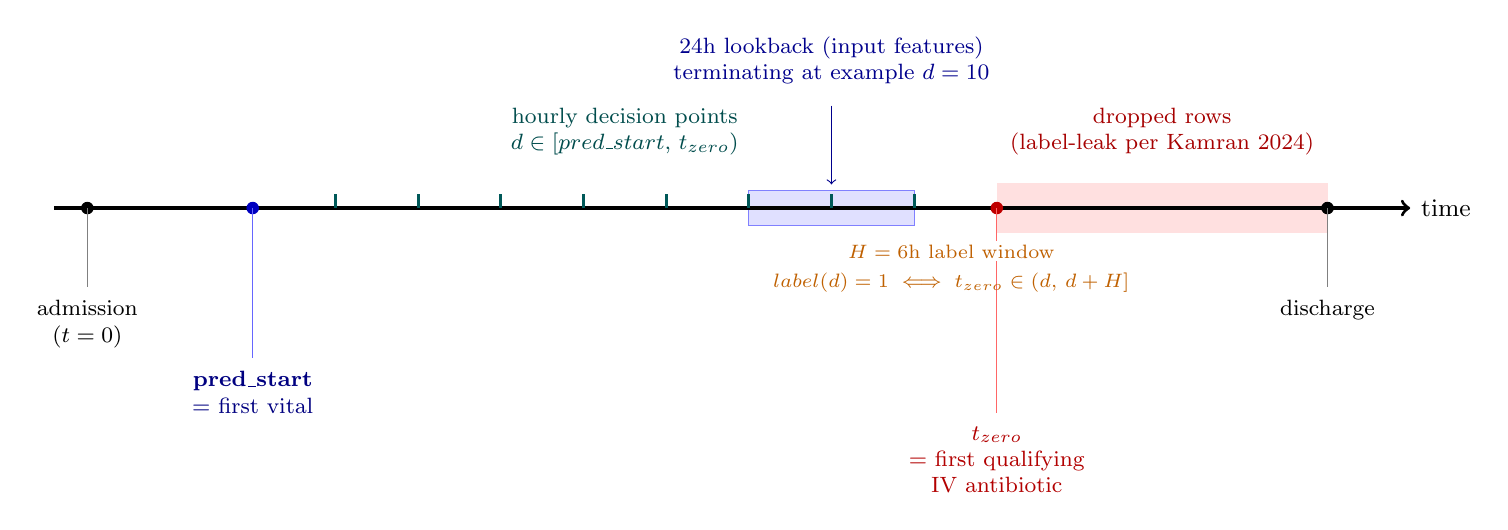
\begin{tikzpicture}[
    x=1.05cm,
    y=1cm,
    every node/.style={font=\small},
    dot/.style={circle, fill=black, inner sep=1.6pt},
    above_lbl/.style={align=center, anchor=south, font=\footnotesize},
    below_lbl/.style={align=center, anchor=north, font=\footnotesize},
    zone/.style={fill=red!12, draw=none},
    look/.style={fill=blue!12, draw=blue!50},
    decision/.style={draw=teal!70!black, line width=1.1pt},
]

    % --- exclusion zone (post-antibiotic) ---
    \fill[zone] (11,-0.32) rectangle (15,0.32);

    % --- 24h rolling lookback box at example decision point d=10 ---
    \fill[look] (8,-0.22) rectangle (10,0.22);

    % --- main time axis ---
    \draw[->, very thick] (-0.4,0) -- (16,0) node[right] {time};

    % --- key anchors with vertical offset labels to avoid collisions ---
    % admission at x=0
    \node[dot] (admit) at (0,0) {};
    \draw[gray] (0,0) -- (0,-1.0);
    \node[below_lbl] at (0,-1.05) {admission\\($t = 0$)};

    % pred_start at x=2.0
    \node[dot, fill=blue!75!black] (vital) at (2,0) {};
    \draw[blue!60] (2,0) -- (2,-1.9);
    \node[below_lbl, text=blue!50!black] at (2,-1.95)
        {\textbf{pred\_start}\\$=$ first vital};

    % t_zero at x=11
    \node[dot, fill=red!75!black] (tzero) at (11,0) {};
    \draw[red!60] (11,0) -- (11,-2.6);
    \node[below_lbl, text=red!70!black] at (11,-2.65)
        {\textbf{$t_{\text{zero}}$}\\$=$ first qualifying\\IV antibiotic};

    % discharge at x=15
    \node[dot] (disch) at (15,0) {};
    \draw[gray] (15,0) -- (15,-1.0);
    \node[below_lbl] at (15,-1.05) {discharge};

    % --- decision-point grid (hourly, schematic) between pred_start and t_zero ---
    \foreach \x in {3,4,5,6,7,8,9,10} {
        \draw[decision] (\x,0) -- (\x,0.18);
    }

    % --- TOP labels (staggered vertical heights) ---
    \node[above_lbl, text=teal!60!black] at (6.5, 0.55)
        {hourly decision points\\$d \in [\text{pred\_start},\, t_{\text{zero}})$};

    \node[above_lbl, text=blue!55!black] at (9, 1.45)
        {24h lookback (input features)\\terminating at example $d=10$};
    \draw[blue!55!black, ->, thin] (9,1.3) -- (9, 0.3);

    \node[above_lbl, text=red!65!black] at (13, 0.55)
        {dropped rows\\(label-leak per Kamran 2024)};

    % --- bottom annotation: label window for example d ---
    \draw[<->, thick, orange!75!black]
        (10, -0.55) -- node[fill=white, inner sep=1.2pt, font=\scriptsize]
        {$H = 6$h label window} (10.9, -0.55);
    \node[font=\scriptsize, orange!75!black, anchor=north]
        at (10.45, -0.7)
        {$\text{label}(d)=1 \iff t_{\text{zero}} \in (d,\, d+H]$};

\end{tikzpicture}
